\section{RESULTS AND DISCUSSION}

\subsection{Geometrical correctness}

The three methods under study achieved good results in
terms of geometrical accuracy. In this ranking, the best
results were obtained with the \gls*{reb} method. Second
best were obtained with \gls*{t2b}. We visually checked
the numbers reported in \autoref{table:results}. 
\autoref{fig:results} shows the B0 volumes after correction.


\subsection{Signal loss recovery}

A second workflow evaluated the different correction methodologies
with analysis of the outcome similarity with respect to the
the original signal. In this second study, \gls*{reb} performed
significantly better than the other two methods, as reported
in \autoref{table:results}.

\subsection{Tractography impact}

Tractography was shown to be deeply influenced by distortion and
the correction method choice. As expected from the scores obtained
by \gls*{reb} in the signal similarity check, this is also the
best ranked method in this category. 

\subsection{Discussion}


\begin{table}[!t]
\caption{Accuracy results}
\label{table:results}
\begin{center}
\begin{tabular}{c||cccc|cc}
\hline
 & \multicolumn{4}{c|}{ Overlap (Jaccard Index, \%)} & \multicolumn{2}{c}{ Signal Correlation (\%)} \\
\hline
 & Av. & \gls*{csf} & \gls*{wm} & \gls*{gm} & \textit{b0} & \glspl*{dwi} \\
\hline
\gls*{fmb} & $93.00$ & $88.57$ & $96.74$ & $94.02$ & $80.05$ & $96.26\pm.06$ \\
\hline
\gls*{reb} & $96.64$ & $94.31$ & $98.26$ & $96.75$ & $91.00$ & $97.65\pm.03$ \\
\hline
\gls*{t2b} & $79.19$ & $66.31$ & $89.85$ & $82.14$ & $64.58$ & $90.10\pm.13$ \\
\hline
\end{tabular}
\end{center}
\end{table}

\begin{figure}[thpb]
   \centering
   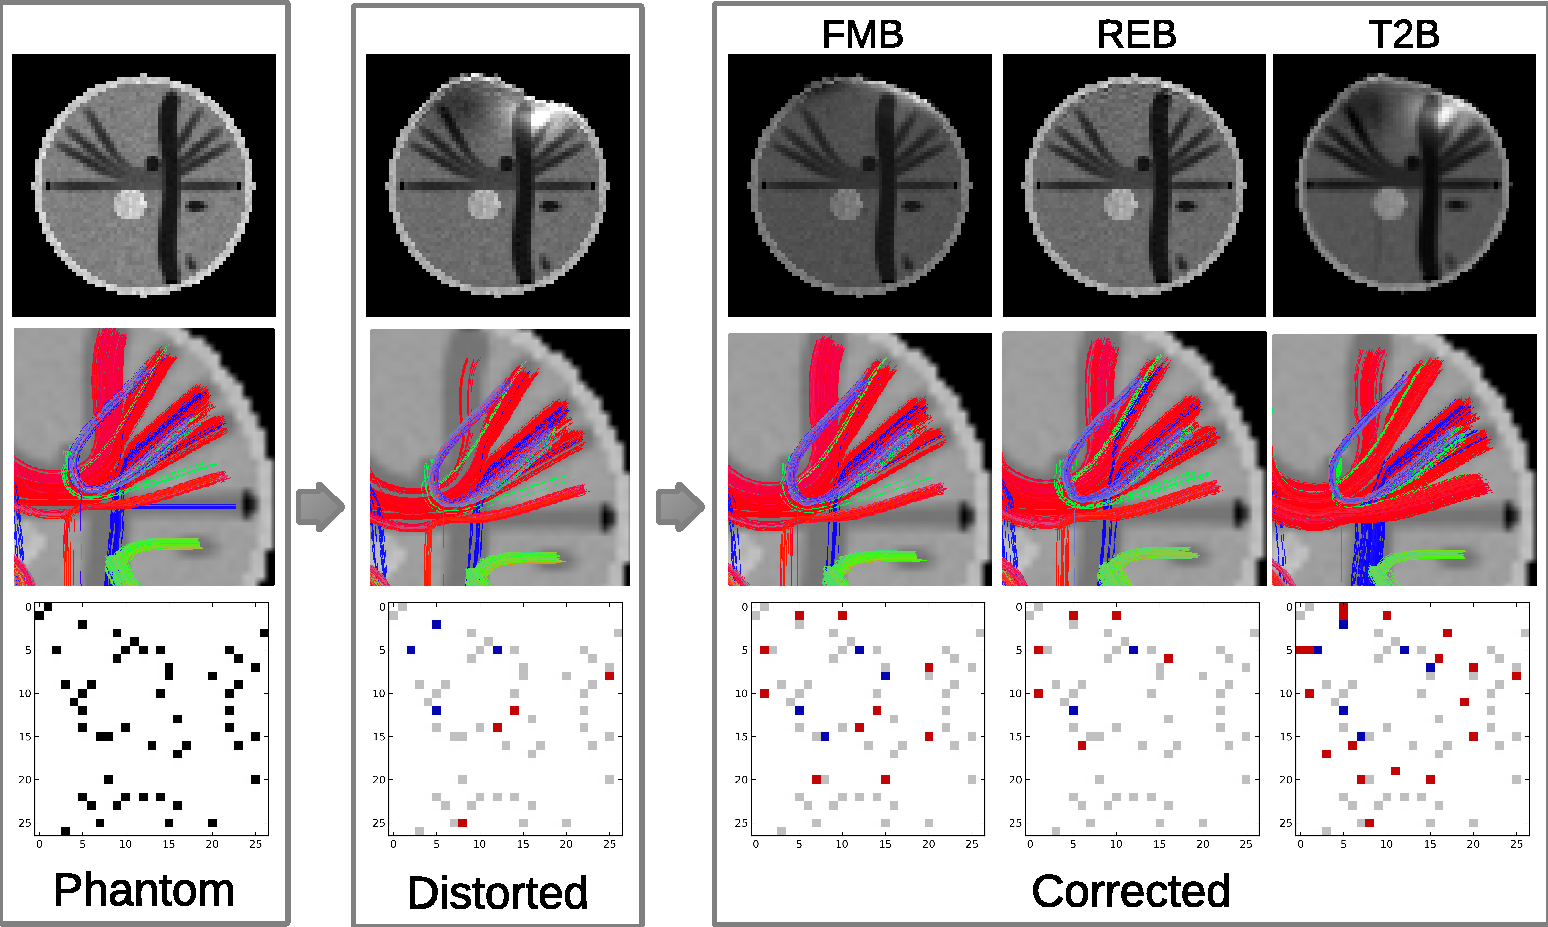
\includegraphics[width=0.8\columnwidth]{Fig02-Results}
   \caption{Visual results}
   \label{fig:results}
\end{figure}

Even though all the surveyed methods produced visually sound results,
\gls*{reb} showed the best results for all the tests. Therefore,
this study suggests that \gls*{reb} is the best available
methodology for susceptibility-induced distortions in
\gls*{epi}. An important limitation of this work is that 
\gls*{psf}-based methods could not be compared, as a
\gls*{psf} map consistent with the synthetic phase-difference
map could not be generated. Nonetheless, to our knowledge there are
no \gls*{psf}-based methods with readily available implementations
for comparison. Moreover, whereas acquiring one extra dataset
among \gls*{t2}, fieldmap, or reversed-encoding B0 is included in
every typical \gls*{dmri} acquisition protocol, the \gls*{psf} 
mapping is not usually performed. Therefore, the most common
correction methodologies are included in the proposed evaluation
framework, along with the benchmarking results.